\documentclass[12pt,a4paper]{article}

% ─── Packages ───
\usepackage[margin=2.5cm]{geometry}
\usepackage{graphicx}
\usepackage{hyperref}
\usepackage{listings}
\usepackage{xcolor}
\usepackage{booktabs}
\usepackage{tabularx}
\usepackage{float}
\usepackage{amsmath}
\usepackage{tikz}
\usetikzlibrary{shapes.geometric, arrows.meta, positioning, fit}
\usepackage{fancyhdr}
\usepackage{titlesec}
\usepackage{enumitem}
\usepackage{caption}
\usepackage{subcaption}
\usepackage[T1]{fontenc}
\usepackage{lmodern}

% ─── Colors ───
\definecolor{codeblue}{HTML}{2196F3}
\definecolor{codegreen}{HTML}{4CAF50}
\definecolor{codered}{HTML}{F44336}
\definecolor{codegray}{HTML}{9E9E9E}
\definecolor{codebg}{HTML}{F5F5F5}
\definecolor{teal}{HTML}{00BFA5}
\definecolor{navy}{HTML}{0A1628}

% ─── Code listing style ───
\lstdefinestyle{codestyle}{
  backgroundcolor=\color{codebg},
  basicstyle=\ttfamily\footnotesize,
  breaklines=true,
  captionpos=b,
  commentstyle=\color{codegreen},
  keywordstyle=\color{codeblue}\bfseries,
  stringstyle=\color{codered},
  numberstyle=\tiny\color{codegray},
  numbers=left,
  numbersep=8pt,
  frame=single,
  rulecolor=\color{codegray!30},
  tabsize=2,
  showstringspaces=false,
}
\lstset{style=codestyle}

% ─── Header/Footer ───
\pagestyle{fancy}
\fancyhf{}
\fancyhead[L]{\textsc{SwiftTrack Middleware}}
\fancyhead[R]{\textsc{System Design Document}}
\fancyfoot[C]{\thepage}
\renewcommand{\headrulewidth}{0.4pt}

% ─── Section formatting ───
\titleformat{\section}{\Large\bfseries\color{navy}}{}{0em}{}[\titlerule]
\titleformat{\subsection}{\large\bfseries\color{navy!80}}{}{0em}{}
\titleformat{\subsubsection}{\normalsize\bfseries\color{navy!60}}{}{0em}{}

% ─── Hyperlink style ───
\hypersetup{
  colorlinks=true,
  linkcolor=codeblue,
  urlcolor=teal,
  citecolor=codegreen
}

% ═══════════════════════════════════════════
\begin{document}

% ─── Title Page ───
\begin{titlepage}
  \centering
  \vspace*{3cm}
  
  {\Huge\bfseries SwiftTrack}\\[0.5cm]
  {\LARGE Event-Driven Middleware for\\Legacy System Integration}\\[2cm]
  
  {\large\textsc{System Design \& Implementation Document}}\\[1cm]
  
  \vfill
  
  \begin{tabular}{rl}
    \textbf{Module:} & Enterprise Application Integration \\
    \textbf{Technology:} & Node.js, Express, RabbitMQ, MongoDB \\
    \textbf{Architecture:} & Microservices with Event-Driven Messaging \\
    \textbf{Repository:} & \url{https://github.com/Kalana2/SwiftLogistics} \\
    \textbf{Date:} & February 2026 \\
  \end{tabular}
  
  \vspace{2cm}
\end{titlepage}

\tableofcontents
\newpage

% ═══════════════════════════════════════════
\section{Introduction}

\subsection{Problem Statement}
Modern logistics organizations depend on multiple legacy systems—Content Management Systems (CMS) using SOAP/XML, Warehouse Management Systems (WMS) using TCP sockets, and Route Optimization Services (ROS) using REST APIs. These systems were designed independently and cannot communicate directly with each other or with modern web clients.

\subsection{Solution Overview}
SwiftTrack is an \textbf{event-driven middleware platform} that integrates these heterogeneous legacy systems through a unified microservice architecture. It uses RabbitMQ as a message broker to orchestrate asynchronous communication, MongoDB for persistence, and Socket.IO for real-time client notifications.

\subsection{Key Objectives}
\begin{enumerate}[leftmargin=2cm]
  \item Provide a unified REST API for all client interactions
  \item Translate between disparate protocols (REST $\leftrightarrow$ SOAP, REST $\leftrightarrow$ TCP)
  \item Ensure reliable message delivery with RabbitMQ
  \item Support real-time order tracking via WebSocket
  \item Implement the Saga pattern for distributed transaction management
\end{enumerate}

% ═══════════════════════════════════════════
\section{System Architecture}

\subsection{Architectural Overview}

\begin{figure}[H]
\centering
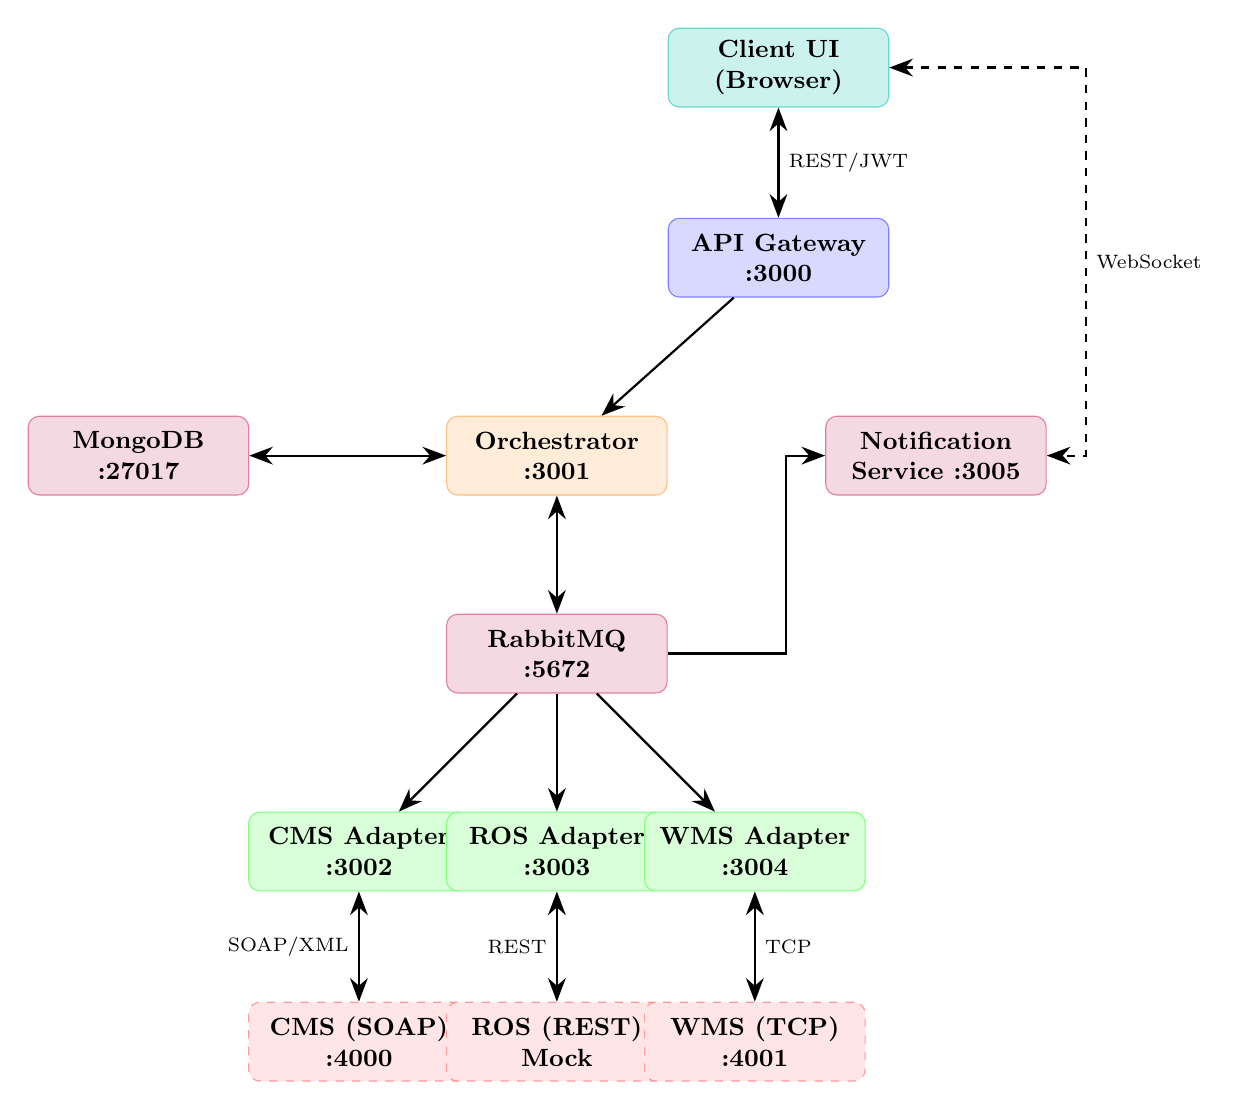
\begin{tikzpicture}[
  node distance=1.4cm and 2.2cm,
  box/.style={rectangle, draw, rounded corners=4pt, minimum width=2.8cm, minimum height=1cm, align=center, font=\small\bfseries},
  client/.style={box, fill=teal!20, draw=teal!60},
  gateway/.style={box, fill=blue!15, draw=blue!50},
  core/.style={box, fill=orange!15, draw=orange!50},
  adapter/.style={box, fill=green!15, draw=green!50},
  legacy/.style={box, fill=red!10, draw=red!40, dashed},
  infra/.style={box, fill=purple!15, draw=purple!50},
  arrow/.style={-{Stealth[length=3mm]}, thick},
  darrow/.style={{Stealth[length=3mm]}-{Stealth[length=3mm]}, thick}
]

% Client layer
\node[client] (ui) {Client UI\\(Browser)};

% Gateway
\node[gateway, below=of ui] (gw) {API Gateway\\:3000};

% Core
\node[core, below left=1.5cm and 0cm of gw] (orch) {Orchestrator\\:3001};
\node[infra, right=2cm of orch] (notif) {Notification\\Service :3005};

% Message broker
\node[infra, below=1.5cm of orch] (rmq) {RabbitMQ\\:5672};

% Adapters
\node[adapter, below left=1.5cm and -0.3cm of rmq] (cms) {CMS Adapter\\:3002};
\node[adapter, below=1.5cm of rmq] (ros) {ROS Adapter\\:3003};
\node[adapter, below right=1.5cm and -0.3cm of rmq] (wms) {WMS Adapter\\:3004};

% Legacy systems
\node[legacy, below=of cms] (cmsl) {CMS (SOAP)\\:4000};
\node[legacy, below=of ros] (rosl) {ROS (REST)\\Mock};
\node[legacy, below=of wms] (wmsl) {WMS (TCP)\\:4001};

% Infrastructure
\node[infra, left=2.5cm of orch] (mongo) {MongoDB\\:27017};

% Arrows
\draw[darrow] (ui) -- node[right, font=\scriptsize] {REST/JWT} (gw);
\draw[arrow] (gw) -- (orch);
\draw[darrow, dashed] (ui.east) -- ++(2.5,0) |- node[right, near start, font=\scriptsize] {WebSocket} (notif);
\draw[darrow] (orch) -- (rmq);
\draw[darrow] (orch) -- (mongo);
\draw[arrow] (rmq) -- (cms);
\draw[arrow] (rmq) -- (ros);
\draw[arrow] (rmq) -- (wms);
\draw[darrow] (cms) -- node[left, font=\scriptsize] {SOAP/XML} (cmsl);
\draw[darrow] (ros) -- node[left, font=\scriptsize] {REST} (rosl);
\draw[darrow] (wms) -- node[right, font=\scriptsize] {TCP} (wmsl);
\draw[arrow] (rmq.east) -- ++(1.5,0) |- (notif);

\end{tikzpicture}
\caption{SwiftTrack System Architecture}
\label{fig:architecture}
\end{figure}

\subsection{Technology Stack}

\begin{table}[H]
\centering
\caption{Technology Stack}
\begin{tabularx}{\textwidth}{lXl}
\toprule
\textbf{Component} & \textbf{Purpose} & \textbf{Technology} \\
\midrule
API Gateway & Authentication, routing, rate limiting & Express, JWT, Helmet \\
Orchestrator & Order lifecycle, business logic & Express, Mongoose \\
Message Broker & Async inter-service communication & RabbitMQ (AMQP) \\
Database & Order persistence & MongoDB \\
CMS Adapter & Legacy CMS integration & SOAP/XML (fast-xml-parser) \\
ROS Adapter & Route optimization & REST (Axios) \\
WMS Adapter & Warehouse management & TCP (net module) \\
Notification Svc & Real-time updates & Socket.IO \\
Client UI & Web dashboard & HTML, CSS, JavaScript \\
\bottomrule
\end{tabularx}
\end{table}

% ═══════════════════════════════════════════
\section{Service Descriptions}

\subsection{API Gateway (Port 3000)}

The API Gateway is the single entry point for all client requests. It handles:

\begin{itemize}[leftmargin=2cm]
  \item \textbf{Authentication}: JWT token generation and verification
  \item \textbf{Authorization}: Role-based access control (client vs driver)
  \item \textbf{Rate Limiting}: 100 requests per minute per IP
  \item \textbf{CORS}: Cross-origin resource sharing for the client UI
  \item \textbf{Request Proxying}: Forwards validated requests to the Orchestrator
\end{itemize}

\begin{lstlisting}[language=java, caption={JWT Authentication Middleware}]
function authenticateJWT(req, res, next) {
  const authHeader = req.headers.authorization;
  const token = authHeader?.split(' ')[1];
  
  if (!token) return res.status(401).json({ error: 'No token' });
  
  try {
    req.user = jwt.verify(token, process.env.JWT_SECRET);
    next();
  } catch (err) {
    return res.status(403).json({ error: 'Invalid token' });
  }
}
\end{lstlisting}

\subsubsection{API Endpoints}

\begin{table}[H]
\centering
\caption{API Gateway Route Map}
\begin{tabularx}{\textwidth}{llX}
\toprule
\textbf{Method} & \textbf{Path} & \textbf{Description} \\
\midrule
POST & /api/auth/login & Authenticate user, return JWT \\
POST & /api/auth/register & Register new user \\
GET & /api/orders & List customer orders \\
POST & /api/orders & Submit new order \\
GET & /api/orders/:id & Get order details \\
GET & /api/driver/manifest & Get driver delivery manifest \\
POST & /api/driver/delivery/:id/status & Update delivery status \\
GET & /health & Service health check \\
\bottomrule
\end{tabularx}
\end{table}

\subsection{Orchestration Service (Port 3001)}

The Orchestration Service is the \textbf{central coordinator} of the order lifecycle. It persists orders in MongoDB and publishes events to RabbitMQ for downstream adapters.

\subsubsection{Order Lifecycle}

\begin{figure}[H]
\centering
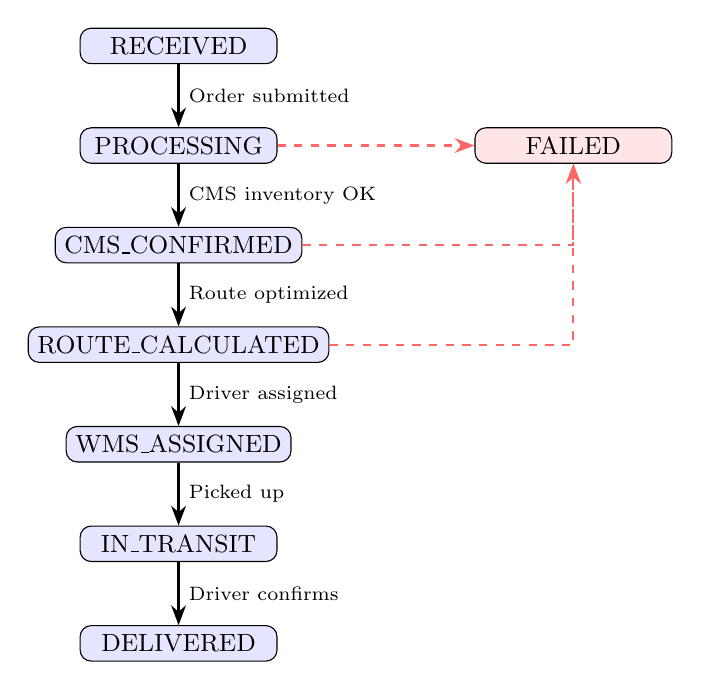
\begin{tikzpicture}[
  state/.style={rectangle, draw, rounded corners, fill=blue!10, minimum width=2.5cm, align=center, font=\small},
  arrow/.style={-{Stealth[length=2.5mm]}, thick},
  node distance=0.8cm
]
\node[state] (recv) {RECEIVED};
\node[state, below=of recv] (proc) {PROCESSING};
\node[state, below=of proc] (cms) {CMS\_CONFIRMED};
\node[state, below=of cms] (route) {ROUTE\_CALCULATED};
\node[state, below=of route] (wms) {WMS\_ASSIGNED};
\node[state, below=of wms] (transit) {IN\_TRANSIT};
\node[state, below=of transit] (deliv) {DELIVERED};

\node[state, right=2.5cm of proc, fill=red!10] (fail) {FAILED};

\draw[arrow] (recv) -- node[right, font=\scriptsize] {Order submitted} (proc);
\draw[arrow] (proc) -- node[right, font=\scriptsize] {CMS inventory OK} (cms);
\draw[arrow] (cms) -- node[right, font=\scriptsize] {Route optimized} (route);
\draw[arrow] (route) -- node[right, font=\scriptsize] {Driver assigned} (wms);
\draw[arrow] (wms) -- node[right, font=\scriptsize] {Picked up} (transit);
\draw[arrow] (transit) -- node[right, font=\scriptsize] {Driver confirms} (deliv);

\draw[arrow, dashed, red!60] (proc) -- (fail);
\draw[arrow, dashed, red!60] (cms) -| (fail);
\draw[arrow, dashed, red!60] (route) -| (fail);

\end{tikzpicture}
\caption{Order Status State Machine}
\label{fig:lifecycle}
\end{figure}

\subsubsection{MongoDB Schema}

\begin{lstlisting}[language=java, caption={Mongoose Order Schema}]
const orderSchema = new mongoose.Schema({
  orderId:    { type: String, required: true, unique: true },
  customerId: { type: String, required: true, index: true },
  items: [{
    sku:      { type: String, required: true },
    name:     String,
    quantity: { type: Number, min: 1 },
    price:    { type: Number, min: 0 }
  }],
  deliveryAddress: {
    street: String, city: String, state: String, zip: String
  },
  status: {
    type: String,
    enum: ['RECEIVED','PROCESSING','CMS_CONFIRMED',
           'ROUTE_CALCULATED','WMS_ASSIGNED',
           'IN_TRANSIT','DELIVERED','FAILED'],
    default: 'RECEIVED'
  },
  metadata: {
    cmsReference: String,
    routeId: String,
    warehouseId: String,
    driverId: String,
    estimatedDelivery: Date
  },
  statusHistory: [{ status: String, timestamp: Date,
                     message: String, source: String }]
}, { timestamps: true });
\end{lstlisting}

\subsection{RabbitMQ Message Architecture}

\begin{table}[H]
\centering
\caption{RabbitMQ Exchanges and Queues}
\begin{tabularx}{\textwidth}{llXl}
\toprule
\textbf{Exchange} & \textbf{Type} & \textbf{Purpose} & \textbf{Routing Keys} \\
\midrule
order\_exchange & topic & Route orders to adapters & order.cms, order.ros, order.wms \\
event\_exchange & fanout & Broadcast events to all & * (all listeners) \\
\bottomrule
\end{tabularx}
\end{table}

\begin{table}[H]
\centering
\caption{Message Queues}
\begin{tabularx}{\textwidth}{lXl}
\toprule
\textbf{Queue} & \textbf{Purpose} & \textbf{Consumer} \\
\midrule
new\_order\_queue & New order submissions & Orchestrator \\
cms\_request\_queue & CMS inventory/confirm & CMS Adapter \\
ros\_request\_queue & Route calculation & ROS Adapter \\
wms\_request\_queue & Warehouse/driver assign & WMS Adapter \\
completed\_order\_queue & Completed orders & Orchestrator \\
notification\_queue & Real-time notifications & Notification Service \\
\bottomrule
\end{tabularx}
\end{table}

\subsubsection{Event Types}

\begin{lstlisting}[language=java, caption={Event Type Definitions}]
const EventTypes = {
  ORDER_RECEIVED:    'order.received',
  ORDER_PROCESSING:  'order.processing',
  ORDER_COMPLETED:   'order.completed',
  ORDER_FAILED:      'order.failed',
  CMS_SUCCESS:       'cms.success',
  CMS_FAILURE:       'cms.failure',
  ROS_SUCCESS:       'ros.success',
  ROS_FAILURE:       'ros.failure',
  WMS_SUCCESS:       'wms.success',
  WMS_FAILURE:       'wms.failure',
  NOTIFICATION_SEND: 'notification.send'
};
\end{lstlisting}

% ═══════════════════════════════════════════
\section{Adapter Layer}

\subsection{CMS Adapter (Port 3002) — SOAP/XML Integration}

The CMS Adapter communicates with the legacy Content Management System over \textbf{SOAP (Simple Object Access Protocol)}. It translates JSON messages from RabbitMQ into XML SOAP envelopes and parses XML responses back.

\subsubsection{SOAP Request Flow}

\begin{enumerate}
  \item Receives \texttt{order.cms} message from RabbitMQ
  \item Builds XML SOAP envelope for inventory check
  \item Sends HTTP POST to CMS at \texttt{/cms/soap}
  \item Parses XML response (\texttt{fast-xml-parser})
  \item If inventory available: sends confirmation SOAP request
  \item Updates order status to \texttt{CMS\_CONFIRMED}
  \item Publishes \texttt{CMS\_SUCCESS} event
\end{enumerate}

\begin{lstlisting}[language=XML, caption={SOAP Inventory Check Request}]
<soap:Envelope xmlns:soap="http://schemas.xmlsoap.org/soap/envelope/"
               xmlns:cms="http://swifttrack.com/cms/2026">
  <soap:Body>
    <cms:CheckInventoryRequest>
      <cms:OrderId>ORD-2026-0001</cms:OrderId>
      <cms:Items>
        <cms:Item>
          <cms:SKU>PROD001</cms:SKU>
          <cms:Quantity>2</cms:Quantity>
        </cms:Item>
      </cms:Items>
    </cms:CheckInventoryRequest>
  </soap:Body>
</soap:Envelope>
\end{lstlisting}

\subsection{ROS Adapter (Port 3003) — REST Integration}

The Route Optimization Service adapter handles route calculation. It supports both external API calls (e.g., Mapbox, Google Maps) and a built-in mock calculation for development.

\subsubsection{Mock Route Calculation}

\begin{lstlisting}[language=java, caption={Mock Route Calculation}]
function calculateMockRoute(origin, destination) {
  const distance = Math.random() * 50 + 5;   // 5-55 km
  const duration = distance * 2.5;            // ~2.5 min/km
  return {
    routeId: `ROUTE_MOCK_${Date.now()}`,
    distance: Math.round(distance * 10) / 10,
    duration: Math.round(duration),
    estimatedDelivery: new Date(
      Date.now() + duration * 60 * 1000
    ).toISOString()
  };
}
\end{lstlisting}

\subsection{WMS Adapter (Port 3004) — TCP Socket Integration}

The WMS Adapter communicates with the Warehouse Management System via a \textbf{raw TCP socket connection}. Messages are newline-delimited JSON.

\subsubsection{TCP Protocol}

\begin{table}[H]
\centering
\caption{WMS TCP Message Types}
\begin{tabularx}{\textwidth}{lX}
\toprule
\textbf{Message Type} & \textbf{Purpose} \\
\midrule
ASSIGN\_WAREHOUSE & Assign nearest warehouse based on delivery destination \\
ASSIGN\_DRIVER & Assign available driver from warehouse \\
UPDATE\_STATUS & Update delivery status (DELIVERED, FAILED) \\
\bottomrule
\end{tabularx}
\end{table}

\begin{lstlisting}[language=java, caption={TCP Client Connection}]
class WMSClient {
  constructor(host, port) {
    this.client = new net.Socket();
    this.buffer = '';
    this.pending = new Map();
  }

  async sendMessage(message) {
    return new Promise((resolve, reject) => {
      const id = Date.now().toString();
      this.pending.set(id, { resolve, reject });
      this.client.write(JSON.stringify(message) + '\n');
    });
  }
}
\end{lstlisting}

% ═══════════════════════════════════════════
\section{Notification Service (Port 3005)}

The Notification Service provides \textbf{real-time WebSocket communication} to connected clients using Socket.IO. It consumes events from the RabbitMQ \texttt{event\_exchange} and broadcasts updates.

\subsection{Notification Channels}

\begin{itemize}
  \item \textbf{Customer notifications}: Order status updates for a specific customer
  \item \textbf{Order-specific notifications}: Updates for subscribed orders
  \item \textbf{Driver notifications}: New assignment and route updates
\end{itemize}

\begin{lstlisting}[language=java, caption={Socket.IO Event Broadcasting}]
socket.on('register', ({ userId, customerId, role }) => {
  if (customerId) socket.join(`customer:${customerId}`);
  if (role === 'driver') socket.join(`driver:${userId}`);
});

// Broadcast order update
io.to(`customer:${customerId}`).emit('order:update', {
  orderId, status, message, timestamp
});
\end{lstlisting}

% ═══════════════════════════════════════════
\section{Client UI}

The frontend is a \textbf{pure HTML/CSS/JavaScript} single-page application with no build tools or frameworks. It uses:

\begin{itemize}
  \item Hash-based routing (\texttt{\#/login}, \texttt{\#/dashboard})
  \item JWT-authenticated API calls
  \item Self-contained inline SVG icons (no CDN dependency)
  \item Automatic mock API fallback when backend is offline
\end{itemize}

\subsection{Pages}

\begin{table}[H]
\centering
\caption{UI Pages}
\begin{tabularx}{\textwidth}{lX}
\toprule
\textbf{Page} & \textbf{Features} \\
\midrule
Login & Email/password form, JWT handling, role-based redirect \\
Client Dashboard & Order statistics, order table, new order modal, order detail panel \\
Driver Dashboard & Delivery manifest, deliver/fail actions, real-time updates \\
\bottomrule
\end{tabularx}
\end{table}

% ═══════════════════════════════════════════
\section{Data Flow}

\subsection{Complete Order Processing Flow}

\begin{enumerate}
  \item \textbf{Client} sends POST \texttt{/api/orders} with JWT token
  \item \textbf{API Gateway} validates JWT, forwards to Orchestrator
  \item \textbf{Orchestrator} persists order in MongoDB (status: \texttt{RECEIVED})
  \item \textbf{Orchestrator} publishes to \texttt{order\_exchange} with key \texttt{order.cms}
  \item \textbf{CMS Adapter} consumes message, sends SOAP request to CMS
  \item \textbf{CMS} checks inventory, returns SOAP response
  \item \textbf{CMS Adapter} updates Orchestrator via REST (status: \texttt{CMS\_CONFIRMED})
  \item \textbf{Orchestrator} publishes to \texttt{order\_exchange} with key \texttt{order.ros}
  \item \textbf{ROS Adapter} calculates route, updates status: \texttt{ROUTE\_CALCULATED}
  \item \textbf{Orchestrator} publishes to \texttt{order\_exchange} with key \texttt{order.wms}
  \item \textbf{WMS Adapter} sends TCP message to WMS for warehouse + driver assignment
  \item \textbf{WMS} assigns, returns via TCP; adapter updates status: \texttt{WMS\_ASSIGNED}
  \item \textbf{Notification Service} receives events, pushes via WebSocket to client
  \item \textbf{Driver} picks up package → status: \texttt{IN\_TRANSIT}
  \item \textbf{Driver} confirms delivery → status: \texttt{DELIVERED}
\end{enumerate}

% ═══════════════════════════════════════════
\section{Design Patterns}

\subsection{Adapter Pattern}
Each legacy system has a dedicated adapter that translates between the internal JSON message format and the external protocol (SOAP, TCP, REST).

\subsection{Saga Pattern}
The order processing uses an orchestration-based saga. If any step fails (e.g., CMS inventory check), compensating transactions are triggered (e.g., cancel CMS reservation).

\subsection{Event-Driven Architecture}
Services communicate asynchronously through RabbitMQ. This provides loose coupling, fault tolerance, and the ability to scale individual services independently.

\subsection{API Gateway Pattern}
A single entry point handles cross-cutting concerns (auth, rate limiting, logging) and routes to internal services.

% ═══════════════════════════════════════════
\section{Security}

\begin{itemize}
  \item \textbf{JWT Authentication}: Stateless token-based authentication with configurable expiry
  \item \textbf{Helmet}: HTTP security headers (XSS, clickjacking, MIME sniffing)
  \item \textbf{Rate Limiting}: 100 requests/minute per IP via \texttt{express-rate-limit}
  \item \textbf{CORS}: Restricted to configured client origin
  \item \textbf{Input Validation}: Server-side validation via \texttt{express-validator}
  \item \textbf{Environment Variables}: Secrets stored in \texttt{.env} files, never committed
\end{itemize}

% ═══════════════════════════════════════════
\section{Deployment}

\subsection{Docker Compose}

All services are containerized via Docker Compose with a shared bridge network:

\begin{lstlisting}[language=bash, caption={Docker Compose Service List}]
services:
  mongodb          # MongoDB 6 — data persistence
  rabbitmq         # RabbitMQ 3 — message broker
  api-gateway      # Express API Gateway
  orchestration-service  # Order orchestrator
  cms-adapter      # SOAP/XML adapter
  ros-adapter      # Route optimization adapter
  wms-adapter      # TCP warehouse adapter
  notification-service   # Socket.IO notifications
  cms-mock         # Mock CMS SOAP server
  wms-mock         # Mock WMS TCP server
\end{lstlisting}

\subsection{Port Allocation}

\begin{table}[H]
\centering
\caption{Service Port Map}
\begin{tabular}{lcl}
\toprule
\textbf{Service} & \textbf{Port} & \textbf{Protocol} \\
\midrule
API Gateway & 3000 & HTTP/REST \\
Orchestrator & 3001 & HTTP/REST \\
CMS Adapter & 3002 & HTTP (health) \\
ROS Adapter & 3003 & HTTP (health) \\
WMS Adapter & 3004 & HTTP (health) \\
Notification Service & 3005 & HTTP + WebSocket \\
CMS Mock & 4000 & HTTP/SOAP \\
WMS Mock & 4001 & TCP \\
MongoDB & 27017 & MongoDB Wire \\
RabbitMQ & 5672 / 15672 & AMQP / Management UI \\
Client UI & 5173 & HTTP (static) \\
\bottomrule
\end{tabular}
\end{table}

% ═══════════════════════════════════════════
\section{Conclusion}

SwiftTrack demonstrates a complete event-driven middleware solution for integrating heterogeneous legacy systems in a logistics domain. The architecture provides:

\begin{itemize}
  \item \textbf{Protocol translation} between SOAP, TCP, and REST
  \item \textbf{Reliable messaging} via RabbitMQ with topic and fanout exchanges
  \item \textbf{Real-time tracking} through Socket.IO WebSocket notifications
  \item \textbf{Fault tolerance} with saga-based compensating transactions
  \item \textbf{Scalability} through independent microservice deployment
  \item \textbf{Security} with JWT authentication and API gateway protection
\end{itemize}

The system successfully bridges the gap between legacy enterprise systems and modern web clients, enabling real-time logistics tracking without modifying the underlying legacy infrastructure.

\end{document}
